\section{1.3 Иные структуры данных}

\subsection{1.3.1 Система Geohash}
Geohash (далее также геохеш) - представляет собой бинарное представление координат (широта-долгота)\cite{jiajunGeohash}. 
Самим геохешем называется строка, закодированная 32 разрядным алфавитом, перевод из 10-ой системы в указанный алфавит указан в таблице 1\cite{sahrIndexingSystems}.
\par\vspace{1em}

\noindent
Таблица 1 --- Алфавит геохеша по основанию 10 и 32
\begin{tabularx}{\textwidth}{ |X|c c c c c c c c| }
 \hline
 Основание 10 & 0 & 1 & 2 & 3 & 4 & 5 & 6 & 7 \\
 Основание 32 & 0 & 1 & 2 & 3 & 4 & 5 & 6 & 7 \\
  \hline
 Основание 10 & 8 & 9 & 10 & 11 & 12 & 13 & 14 & 15 \\
 Основание 32 & 8 & 9 & b & c & d & e & f & g \\
  \hline
 Основание 10 & 16 & 17 & 18 & 19 & 20 & 21 & 22 & 23  \\
 Основание 32 & h & j & k & m & n & p & q & r \\
  \hline
 Основание 10 & 24 & 25 & 26 & 27 & 28 & 29 & 30 & 31 \\
 Основание 32 & s & t & u & v & w & x & y & z \\
  \hline
\end{tabularx}
\par\vspace{1em}
\par\vspace{1em}

Данная строка однозначно декодируется в кортеж координат с точностью, зависящей от количества символов в строке. Примеры:
\par а) строка \texttt{ucft} декодируется в прямоугольник площадью примерно 800 $ km^2 $ и центром в (55.81, 37.44);
\par б) строка \texttt{ucft943} имеет тот же центр - (55.8236, 37.3116), но меньшую площадь --- $23409 m^2$.
Как можно наблюдать, чем выше количество символов, используемых в геохеше, тем выше точность получаемых координат, но при этом выше затрачиваемая память\cite{sidorovGeohash}.
В данной работе не будет детально описываться процесс формирования геохеша за исключением базового принципа.

Сфера земли разбивается на прямоугольники (не обязательно равные), после чего каждому прямоугольнику присваивается номер в 32х-ричной системе координат, номера присваиваются в порядке змейкой, сначала самый левый верхний, далее ниже от него, далее справа от самого левого верхнего и тд, пример разбиения виден на рисунке 5.
\par\vspace{1em}
\begin{figure}[H]
    \centering
    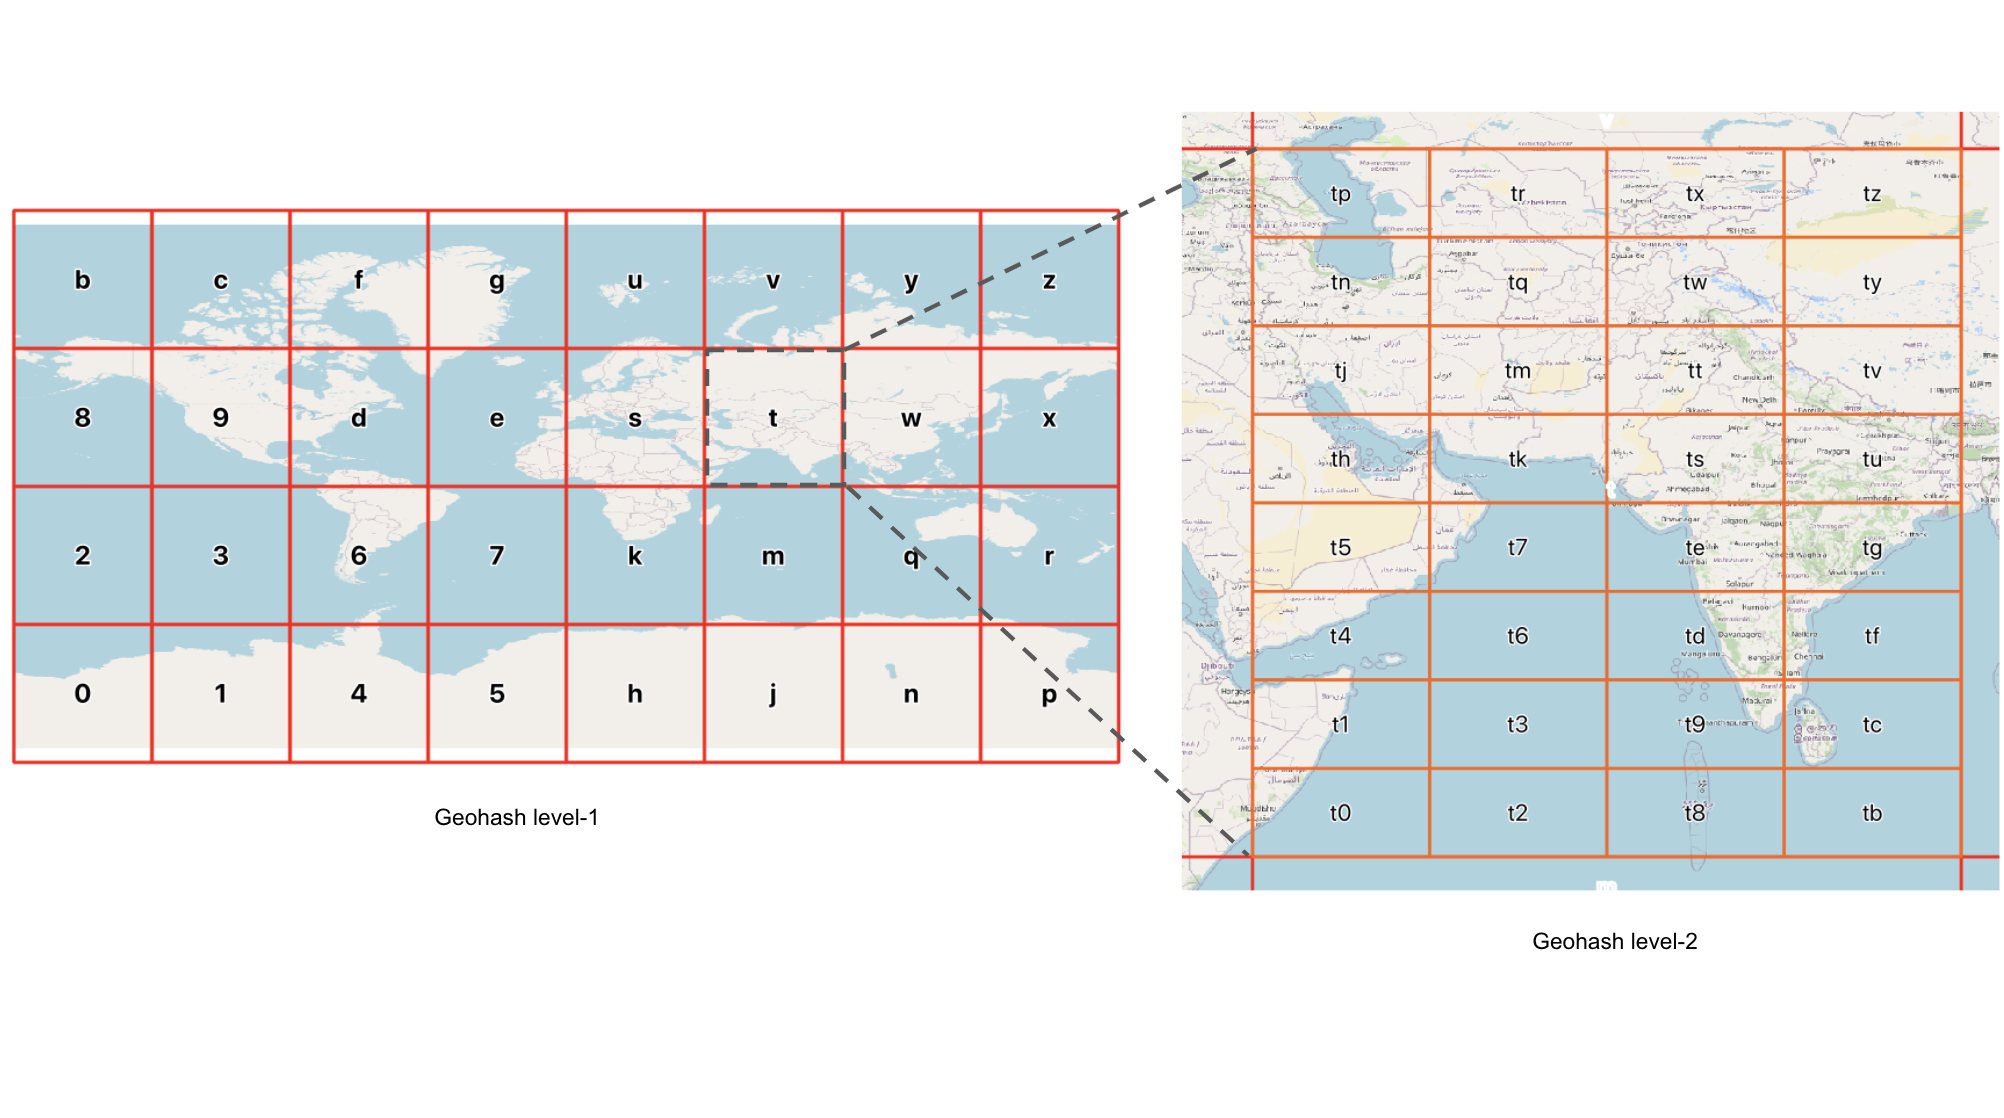
\includegraphics[scale=0.2]{geohash.png}
    \caption{Пример разбиения сферы земли через Geohash на первые 2 префикса}
\end{figure}

Сам по себе Geohash, как и ниже описанные структуры Uber H3 и S2 - не являются индексами\cite{balkicGeohash}, а лишь методами сериализации координат. Реализации алгоритмов поиска на этих методах производится в связке с такими структурами как B-tree, Trie и тд. 

\subsection{1.3.2 Система Uber H3}
Uber H3 - это сетка гексагональных ячеек (рисунок 6), разработанная в компании Uber. Она используется для сериализации и хранения геоданных. Каждая ячейка имеет уникальный идентификатор и может быть использована для определения местоположения объектов. Логика работы Uber H3 аналогична логике Geohash за основным исключением, что в Uber H3 используются шестиугольники, а в Geohash - прямоугольники. 
  \\
\begin{figure}[H]
    \centering
    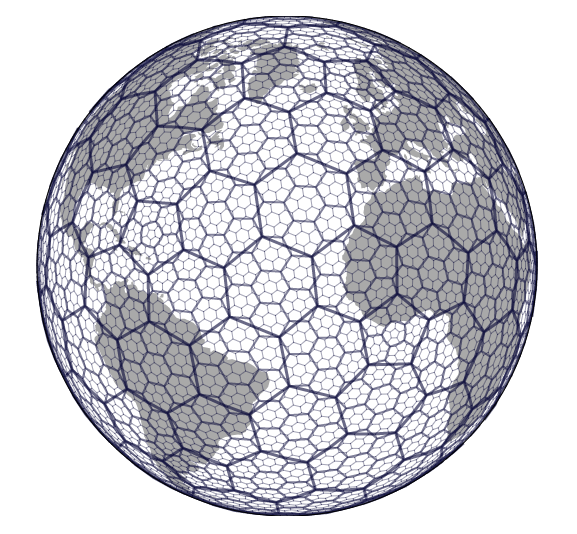
\includegraphics[scale=0.2]{h3.png}
    \caption{Разбиение сферы земли на шестиугольники при использовании H3}
\end{figure}

Принципиальных отличий между H3 и Geohash\cite{bohuiGeohashH2S2}, помимо, конечно, разницы в форме - нет. Оба формата в конечном итоге кодируют данные в бинарном виде, имеется возможность перевести данные в строковое представление.  

Важно отметить, что с точки зрения разработчика, различия все-таки имеются:
\par а) geohash более прост в реализации и понимание его человеком;
\par б) geohash поддерживается такими СУБД, как: Postgis, Redis, Tile38, MongoDB\cite{membreyMongodb};
\par в) H3 имеет очень обширную библиотеку с дополнительными методами;
\par г) H3 поддерживается такими СУБД, как: Clickhouse.

\subsection{1.3.3 Система S2 geometry}

S2 Geometry - это библиотека для работы с геометрическими объектами на сфере, разработанная компанией Google. 
\par\vspace{1em}
\begin{figure}[H]
    \centering
    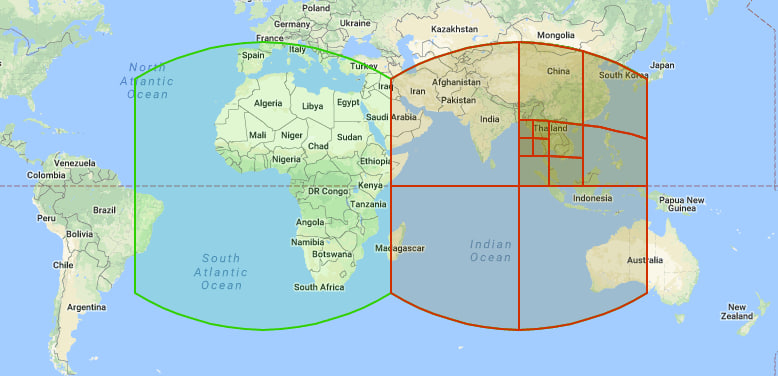
\includegraphics[scale=0.8]{s2-geometry.jpg}
    \caption{Пример разбиения пространства на области с использованием S2 Geometry}
\end{figure}
\par\vspace{1em}

Основой S2 Geometry является иерархическая структура данных, называемая S2 Cell. Как показано на рисунке 7, каждая ячейка S2 Cell представляет собой квадрат на сфере, который может быть разбит на более мелкие квадраты более высокого уровня. Уровень ячейки определяется числом n, которое указывает на количество разбиений квадрата на подквадраты. Чем больше значение n, тем меньше размер каждой ячейки.

S2 не имеет значимых качественных или количественных преимуществ перед Geohash и H3. Также, данный алгоритм имеет довольно скудное представление в СУБД, а также в подключаемых библиотеках в различных языках программирования. 
Из-за перечисленных выше причин данный алгоритм не будет далее рассматриваться в этой работе. 